\documentclass[handout]{beamer}\mode<presentation>{\usetheme{AMSCesenaBleu}}

\usepackage{multicol}
\usepackage{common}
\usepackage{pgfpages}
\usepackage{subfigure}
\usepackage{media9}
\usepackage{xargs} % Use more than one optional parameter in a new commands % Coloured text etc.
\usepackage[colorinlistoftodos,prependcaption]{todonotes}

\newcommandx{\unsure}[2][1=]{\todo[linecolor=red,backgroundcolor=red!25,bordercolor=red,#1]{#2}}
\newcommandx{\change}[2][1=]{\todo[linecolor=blue,backgroundcolor=blue!25,bordercolor=blue,#1]{#2}}
\newcommandx{\improvement}[2][1=]{\todo[linecolor=ForestGreen,backgroundcolor=ForestGreen!25,bordercolor=ForestGreen,#1]{#2}}
\newcommandx{\marianiSays}[2][1=]{\todo[linecolor=Orange,backgroundcolor=Orange!25,bordercolor=Orange,#1]{#2}}

%\setbeameroption{show notes on second screen=right}

% \graphicspath{{res/img/}}

%\AtBeginSection[]
%{
%\begin{frame}<beamer>[c]\frametitle{A seguire\ldots}
%		\tableofcontents[currentsection,hideallsubsections]
%\end{frame}
%}

\newenvironment{nscenter}
{\parskip=1pt\par\nopagebreak\centering}
{\par\noindent\ignorespacesafterend}

\title[Synapsis: Middleware per GE e MAS]{Synapsis - Middleware per l'integrazione di Game Engine e Sistemi Multi-Agente}
\author[Luca Pascucci]{Tesi in: Sistemi Autonomi\\[0.5cm]\textit{Relatore:} \hspace{6cm} \textit{Presentata da:} \\ Chiar.mo Prof. \hspace{4.40cm} Luca Pascucci\\ Andrea Omicini \hspace{7.2cm} \phantom{g} \\\textit{Correlatore:} \hspace{7.75cm} \phantom{g}\\Dott. Stefano Mariani \hspace{6.1cm} \phantom{g}}
\institute[]{
\textsc{Alma Mater Studiorum} -- Università di Bologna \\
Campus di Cesena}
\date{10 Ottobre 2019}

\begin{document}

\maketitle

%\begin{frame}[c]
%\frametitle{Indice}
%	\tableofcontents[hideallsubsections]
%\end{frame}


\section{Introduzione e stato dell'arte}

\subsection{Introduzione}

\begin{frame}
\frametitle[Introduzione e stato dell'arte]{L'obiettivo della tesi}
\begin{block}{Fase 1}
Studiare lo stato dell'arte delle Game Engine (GE) e dei Sistemi Multi-Agente (MAS)
\end{block}
\begin{block}{Fase 2}
Analizzare i due sistemi con lo scopo di:
\begin{itemize}
    \item Evidenziare opportunità per colmare le lacune concettuali/tecniche dei due mondi
    \item Rilevare astrazioni e meccanismi che forniscono supporto nel riformulare le astrazioni mancanti del MAS e della GE
\end{itemize}
\end{block}
\begin{block}{Fase 3}
Proporre un’infrastruttura di associazione e comunicazione tra MAS e GE, rispettandone il disaccoppiamento e l’integrità concettuale delle astrazioni.
\end{block}
\end{frame}

\subsection{Stato dell'arte}

\begin{frame}
\frametitle[Introduzione e stato dell'arte]{Concetti preliminari}
\begin{block}{Sistema Multi-Agente}
Paradigma general-purpose utilizzato per realizzare sistemi complessi. Le astrazioni principali sono:
\begin{itemize}
    \item Agenti: Entità autonome in grado di comunicare, possono essere situati, intelligenti;
    \item Società: Gruppo di agenti che cooperano / competono per realizzare goals;
    \item Ambiente: Il "contenitore" in cui gli agenti eseguono, che li influenza e ne viene influenzato.
\end{itemize}
\end{block}

\begin{block}{Game Engine}
Struttura general-purpose multipiattaforma orientata verso ogni aspetto della progettazione e dello sviluppo di videogiochi
\end{block}

\end{frame}

\section{Stack Tecnologico}

\subsection{Sistema Multi-Agente}

\begin{frame}
\frametitle[Stack Tecnologico]{JaCaMo}

Framework per la programmazione orientata agli agenti che combina tre tecnologie già affermate e sviluppate da diversi anni

\begin{block}{Jason}
Piattaforma di sviluppo agenti basati sull'architettura BDI, implementa AgentSpeak(L).
\end{block}

\begin{block}{CArtAgO}
Modello per la progettazione dell'ambiente MAS, basato sul concetto di workspace ed artefatti.
\end{block}

\begin{block}{Moise}
Meta-modello organizzativo per MAS basato sulle nozioni di ruoli, gruppi e missioni.
\end{block}

\end{frame}

\subsection{Game Engine}

\begin{frame}
\frametitle[Stack Tecnologico]{Unity}

Game Engine cross-platform utilizzata per la creazione di videogiochi (sia 2D che 3D), ambienti virtuali e simulazioni interattive.
\begin{figure}
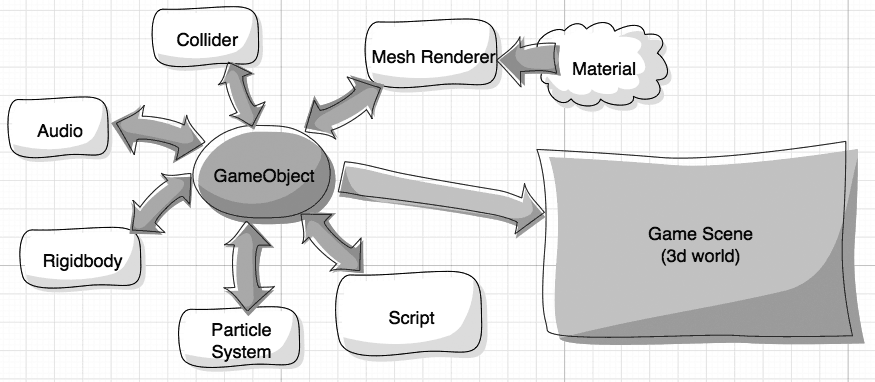
\includegraphics[width=0.8\linewidth]{figures/unity_diagram.png}
\end{figure}

\end{frame}

\section{Terminologia e Modelli computazionali}

\subsection{Terminologia}

\begin{frame}
\frametitle[Stack Tecnologico]{Astrazioni concettuali}

    \begin{block}{Entità}
        Componente divisibile in due parti, mente e corpo, che collegate riescono a trasmettersi informazioni utilizzate dalla mente per raggiungere i propri obiettivi e dal corpo per diventare "attivo" nell’ambiente in cui si trova.
    \end{block}

    \begin{exampleblock}{Corpo}
        Componente associato alla nozione di GameObject per avere una rappresentazione fisica dell’entità da realizzare.
    \end{exampleblock}

    \begin{exampleblock}{Mente}
        Componente autonomo che interagisce con l’ambiente per svolgere i propri compiti associato alla nozione di Agente.
    \end{exampleblock}

\end{frame}

\subsection{Modelli computazionali}

\begin{frame}
\frametitle[Stack Tecnologico]{Integrazione concettuale}

\begin{block}{Agente BDI}
    Focus sul concetto di \alert{Belief} e \alert{Action}
\end{block}

\begin{block}{Artefatto}
    Focus sul concetto di \alert{Proprietà Osservabile} e \alert{Operazione}
\end{block}

\begin{figure}
    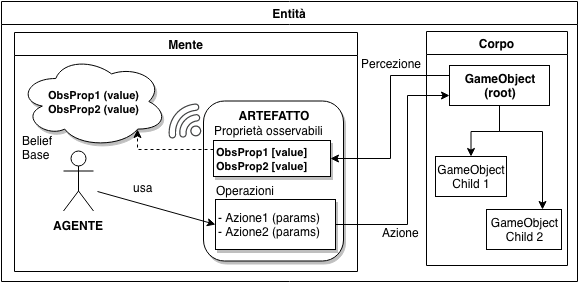
\includegraphics[width=0.8\linewidth]{figures/Ridefinizione_entita.png}
\end{figure}

\end{frame}

\section{Synapsis, Liberie JaCaMo e Unity}

\subsection{Synapsis}

\begin{frame}
\frametitle[Synapsis, Liberie JaCaMo e Unity]{Middleware Synapsis}

\begin{block}{Architettura di sistema}
{\small Sistema ad Attori (Akka, Play)}
{\footnotesize \begin{itemize}
    \item attori = entità computazionali (re)attive
    \item message passing = asincronia, mailbox
    \item fault-tolerance, scalabilità
\end{itemize}}

\end{block}

\begin{figure}
    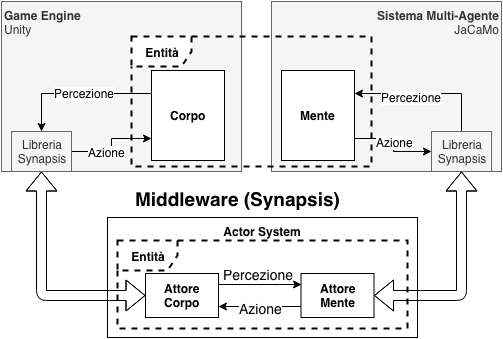
\includegraphics[width=0.5\linewidth]{figures/Middleware_associazione_entita.png}
\end{figure}

\end{frame}

\subsection{Libreria JaCaMo}

\begin{frame}[fragile]

\frametitle[Synapsis, Liberie JaCaMo e Unity]{Synapsis: JaCaMo client}

\begin{minipage}{0.48\linewidth}
    \centering
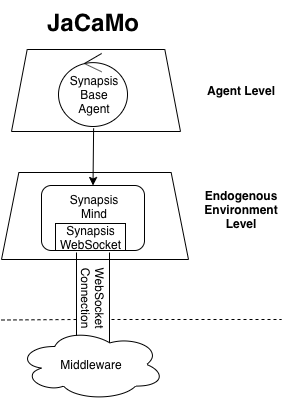
\includegraphics[width=0.75\textwidth]{figures/struttura_libreria_JaCaMo.png}
\end{minipage}
\begin{minipage}{0.48\linewidth}
    \begin{block}{Contenuto}
    \begin{itemize}
        \item Agente "SynapsisBaseAgent"
        \item Arfetatto "SynapsisMind"
    \end{itemize}
    \end{block}
    \begin{block}{API}
    \begin{itemize}
        \item Invio azione generica
        \item Presenza di azioni già delineate (Trova, Vai a, Prendi ...)
        \item Gestione delle percezioni ricevute dal corpo
        \item Connessione WebSocket al middleware
    \end{itemize}
    \end{block}
\end{minipage}

\end{frame}

\subsection{Libreria Unity}

\begin{frame}[fragile]
\frametitle[Synapsis, Liberie JaCaMo e Unity]{Synapsis: Unity client}
\begin{minipage}{0.48\linewidth}
    \centering
    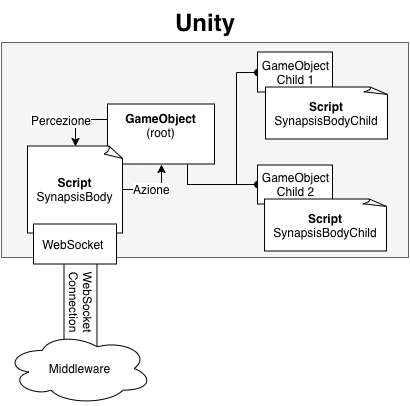
\includegraphics[width=0.8\textwidth]{figures/struttura_libreria_unity.png}
\end{minipage}
\begin{minipage}{0.48\linewidth}
    \begin{block}{Contenuto}
    \begin{itemize}
        \item Script "SynapsisBody"
        \item Script "SynapsisBodyChild"
    \end{itemize}
    \end{block}
    \begin{block}{API}
    \begin{itemize}
        \item Invio percezione generica
        \item Presenza di percezioni già delineate (Trovato, Arrivato, Preso ...)
        \item Invio automatico di percezioni fisiche (contatto con altri oggetti in scena)
        \item Connessione WebSocket al middleware
    \end{itemize}
    \end{block}
\end{minipage}
\end{frame}

\subsection{Architettura totale}

\begin{frame}
\frametitle[Synapsis, Liberie JaCaMo e Unity]{Synapsis: zoom architettura}

\begin{figure}
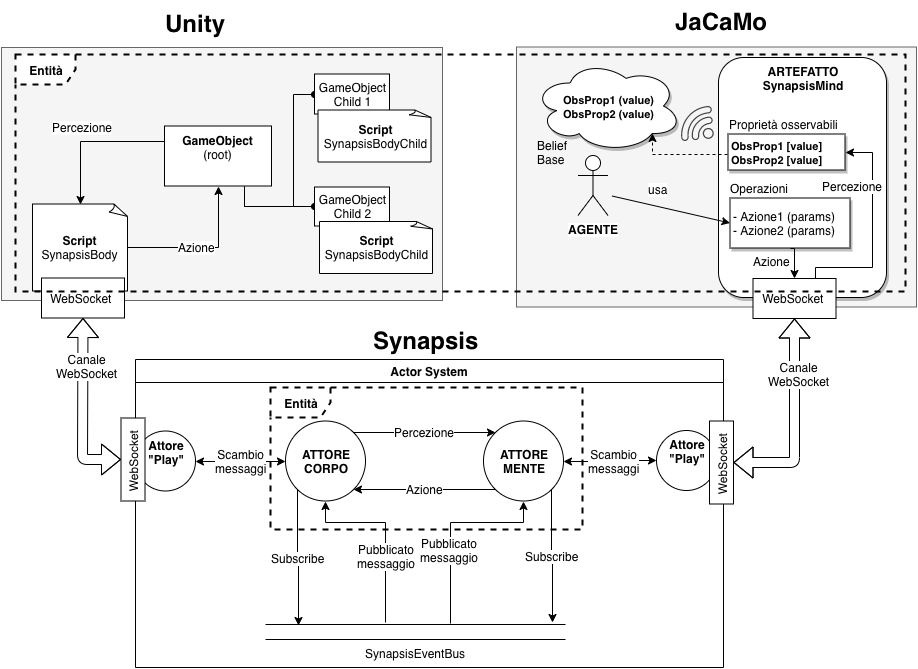
\includegraphics[width=0.8\linewidth]{figures/Synapsis.png}
\end{figure}

\end{frame}

\section{Caso di studio, conclusioni e sviluppi futuri}

\subsection{Caso di studio}

\begin{frame}
\frametitle[Conclusioni e sviluppi futuri]{Recycling Robots}

Scenario contenente robot con il compito di riciclare la spazzatura presente nell'ambiente portandola al rispettivo bidone.


\begin{figure}
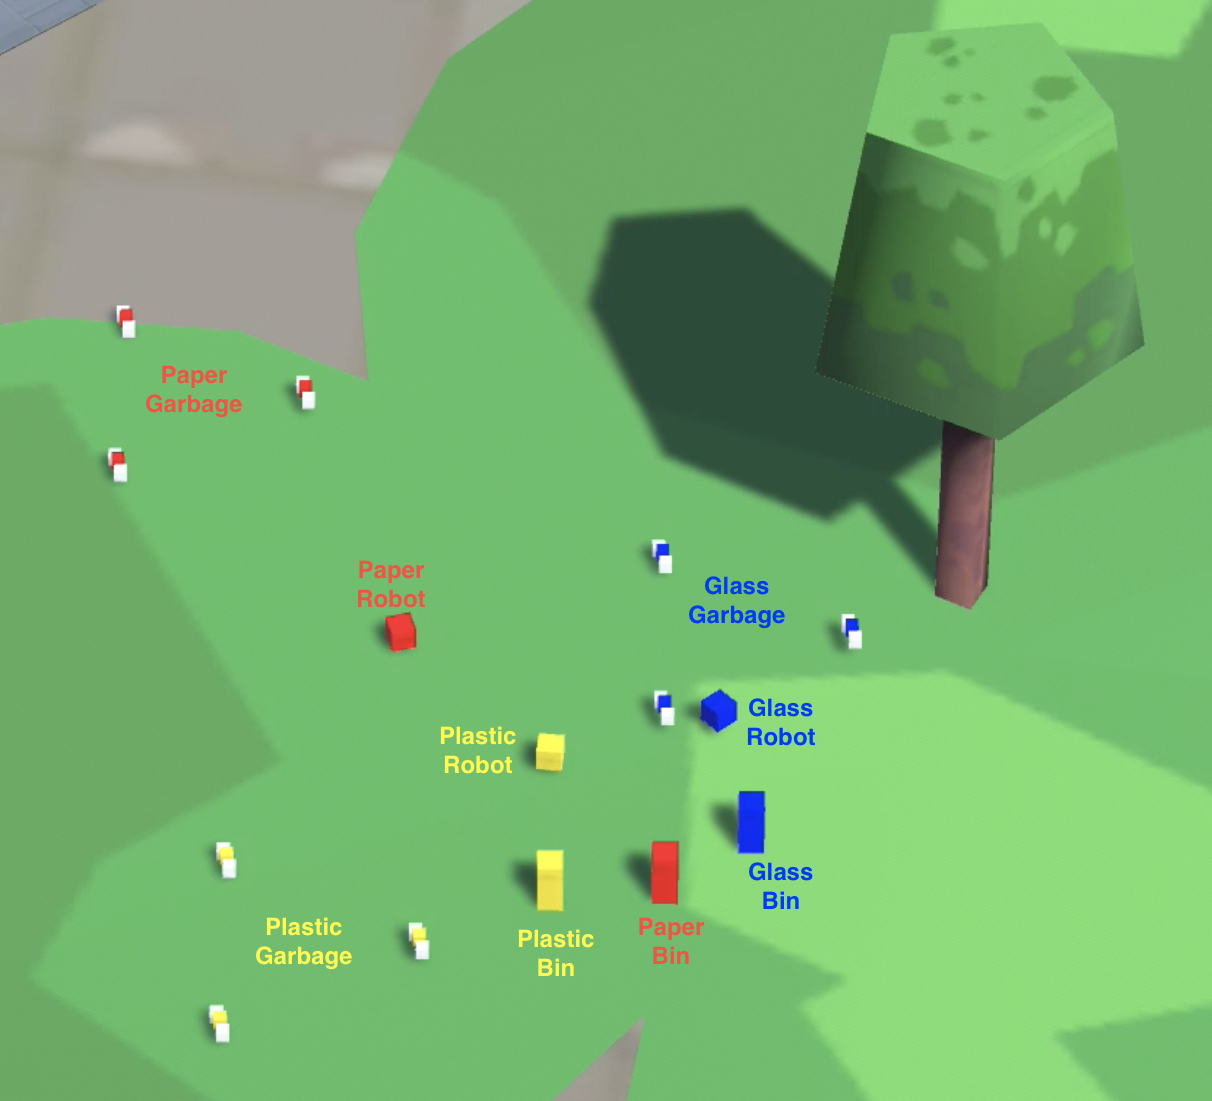
\includegraphics[width=0.5\linewidth]{figures/recycling_robots.png}
\end{figure}

\end{frame}

\subsection{Conclusioni e sviluppi futuri}

\begin{frame}
\frametitle[Conclusioni e sviluppi futuri]{Riassumendo\ldots}

	\begin{block}{Conclusioni}
		\begin{itemize}
         \item Definite linee guida per l'integrazione di Game Engine e Sistemi Multi-Agente
         \item Realizzato middleware e librerie che permettono la costruzione di scenari relativamente complessi
		\end{itemize}
	\end{block}

	\begin{block}{Possibili sviluppi futuri}
		\begin{itemize}
         \item Integrare il modello di coordinazione degli agenti tramite spazio di tuple e primitive Linda
         \item Realizzare nuove librerie per espandere la lista di GE e MAS collegabili
         \item Utilizzare le caratteristiche dei sistemi presenti per realizzare lo stesso scenario distribuito su più elaboratori
		\end{itemize}
	\end{block}

\end{frame}

\maketitle

\end{document}
